\chapter{Português Estruturado - PORTUGOL}
\section{Versão Inicial}
\begin{figure}[!h]
\vspace{-10mm}
    \centering
    \caption{ Está é a versão inicial do nosso Portugol}
    \label{fig:enter-label}
    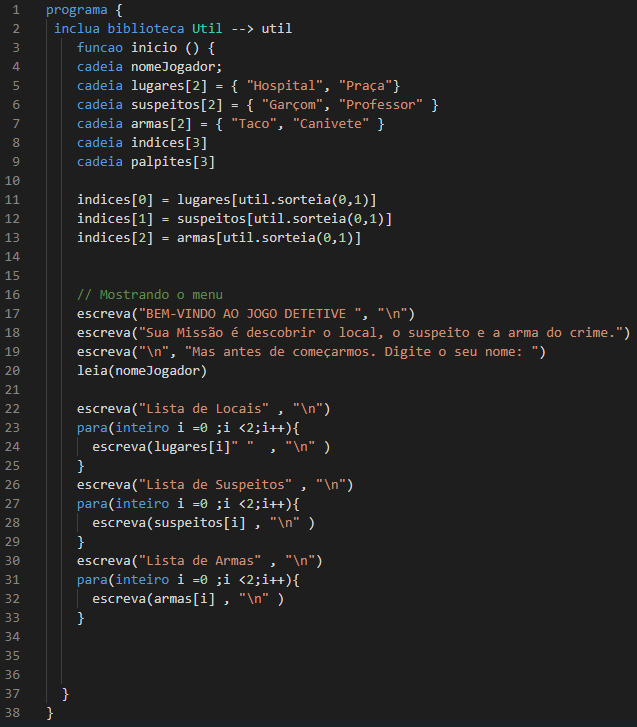
\includegraphics[scale=0.75]{print 2.png }   
    \vspace{8mm}
    \newline
   {\large Quais foram as primeiras ideais para o projeto?}
   
   \begin{flushleft}
 Sortear um vetor com armas, suspeitos e locais aleatorios. Onde o usuario teria que acertar.
\end{flushleft}

 {\large Apresente uma explicação detalhada de cadas método.}
 \begin{flushleft}
.Na versão inicial temos apenas um método para mostrar o menu para o jogador.
\end{flushleft}   
\end{figure}
\pagebreak
\section{Versão Final}

\vspace{-65mm}
\begin{figure}[!h]
    \centering
    \caption{Caption}
    \label{fig:enter-label}
    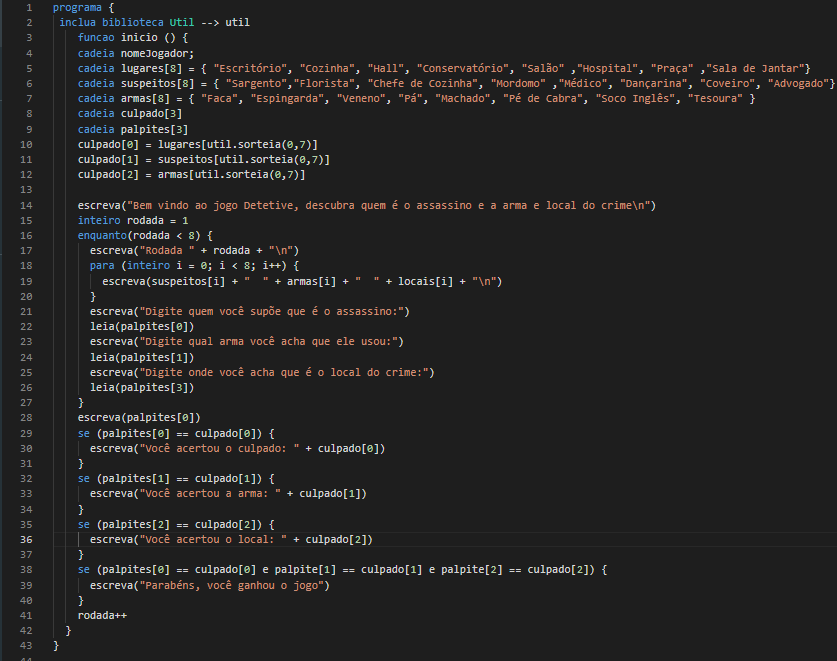
\includegraphics[scale=0.75]{final.png }    


{\large Quais forams os problemas encontrados na versão inicial? }
\newline

\begin{flushleft}
    Não conseguimos fazer a validação do suspeito, armas e locais que o usuario informou.
\end{flushleft}

{\large Quais foram as principais alterações nos métodos da versão final? }
\newline
     \begin{flushleft}
     Conseguimos colocar um sistema de validação dos palpites do usuário de forma visual com cores para indicar se houve acerto ou erro.
\end{flushleft}

{\large Descreva detalhadamente os métodos novos presentes na versão final?}

\end{figure}
\pagebreak

